\documentclass[a4paper,11pt]{article}
\usepackage[utf8x]{inputenc}
% \usepackage[latin1]{inputenc}
% \usepackage[brazil]{babel}
\usepackage[pdftex]{color,graphicx}
\usepackage[a4paper,left=2.2cm,right=2.3cm,top=3.1cm,bottom=3.3cm]{geometry}
\usepackage{subfig}
\usepackage{picinpar}
\usepackage{multicol}
\usepackage{bm}
% \usepackage{program}
\usepackage{varwidth}
\usepackage{parskip}
\usepackage{algorithm}
\usepackage{algpseudocode}
\usepackage{hyperref}
\usepackage{natbib}
\usepackage{url}
\usepackage{pbox}
\usepackage{footnote}




\title{ Classificando spams em uma pequena base \\ de dados de mensagens SMS}

\author{Renzo A. Viloche Morales \\ \texttt{renvmorales@gmail.com}}


\begin{document}

\DeclareGraphicsExtensions{.jpg,.pdf,.mps,.png}
\maketitle

\section{Introdução}

Mineração de texto é comumente usada com a finalidade de analisar e obter uma descrição geral em 
dados não-estruturados (por exemplo, um texto único, ou mensagens enviadas a partir de vários 
usuários). Este tipo de operação não é apenas importante para fins de uma análise exploratória, 
mas também necessário durante a etapa de pré-processamento que fornecerá dados de entrada para 
treinar um modelo (algoritmo) de classificação através de uma técnica de aprendizado de máquina. 

Neste trabalho, uma pequena base de dados de 5.574 mensagens SMS contendo spams (mensagens 
consideradas fora do interesse do destinatário) é analisada brevemente e convertida numericamente 
usando a técnica de idf (?). Uma vez concluído o processamento, a base de dados será separada 
em ``teste'' e ``treinamento'' onde um modelo regressão logística e de redes neurais artificiais 
serão utilizados para classificação (?). Análises, teste e validação de performance dos modelos
foram todos realizados usando a linguagem de código aberto Python, especificamente os módulos: 
\textit{Numpy, Pandas, Scikit-learn, wordcloud}.


% Text mining is commonly used to provide some general description into unustructured data 
% (e.g, single text or multiple collected user messages). This operation is important not just for 
% exploratory data analysis purposes, but also when performing a preprocesing step required in order 
% to apply a machine learning technique such as a classification algorithm. Here a small dataset of 
% SMS messages is analyzed and prepared.



\section{Metodologia}



\section{Resultados}

\subsection{Descrição da base de dados}

A base de dados contida no arquivo \texttt{SMS.csv} é composta por diversas mensagens comuns (4.827)
e spams (747) em inglês dispostos na forma de 5.574 linhas e 154 colunas. Os atributos (cada coluna) 
da base de dados são descritos a seguir:

\begin{itemize}
 \item 1 coluna contendo a mensagem original (\texttt{Full\_Text});
 \item 149 colunas com valores inteiros que indicam a frequência de uma determinada palavra na 
 mensagem (\texttt{got ... wan});
 \item 1 coluna contendo a quantidade de palavras frequentes na mensagem 
 (\texttt{Common\_Words\_Count});
 \item 1 coluna contendo a quantidade total de palavras da mensagem (\texttt{Word\_Count});
 \item 1 coluna contendo a data de recebimento da mensagem (\texttt{Date});
 \item 1 coluna que identifica se a mensagem é spam ou não (\texttt{IsSpam}).
\end{itemize}

Sempre que possível, a base de dados neste trabalho será referida de \texttt{SMS}.


\subsection{Análise exploratória}

Inicialmente foi realizado uma análise das palavras mais frequentes em toda a base. Para isto, 
as frequências totais de cada uma das 149 palavras mais comuns foram calculadas. O seguinte gráfico 
de barras na figura \ref{fig:barplot} exibe cada uma das frequência para palavras com frequência de 
no mínimo igual a 150.

\begin{figure}[htbp]
    \centering
    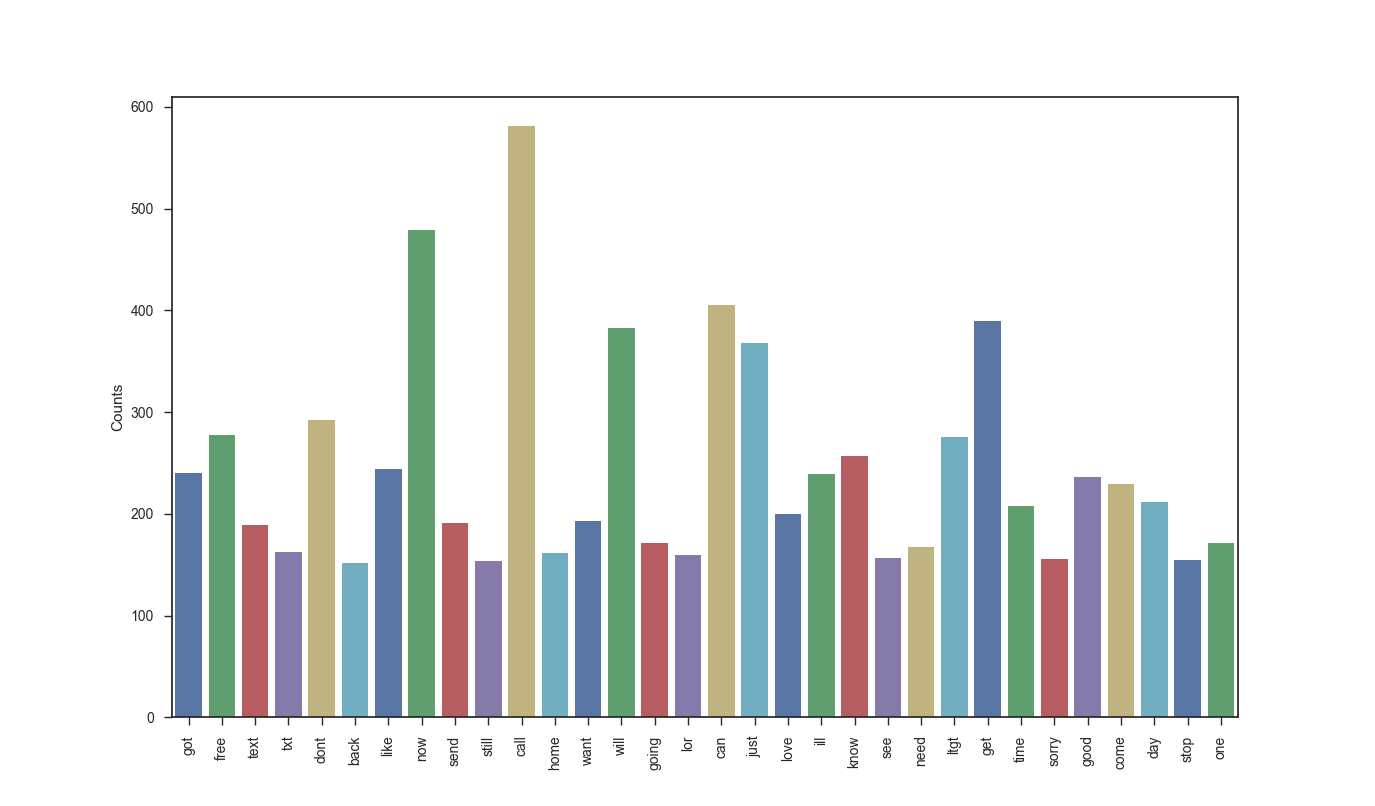
\includegraphics[width=\textwidth]{word_barplot.png}
    \caption[Figura simples]{Gráfico de barras com frequências de palavras mais comuns de 
    \texttt{SMS} superiores a 150.}
    \label{fig:barplot}
\end{figure}

O gráfico mostra 32 palavras com ocorrência superior ao mínimo estabelecido (para efeito de melhor
visualização). A lista completa destas palavras é: \texttt{got, free, text, txt, dont, back, 
like, now, send, still, call, home, want, will, going, lor, can, just, love, ill, know, see, need, 
ltgt, get, time, sorry, good, come, day, stop, one}.

Um outro recurso de mais fácil visualização é a nuvem de palavras. Nela, o tamanho de cada palavra 
é proporcional a sua frequência de ocorrência. Neste caso uma nuvem de palavras foi aplicada sobre 
o universo de palavras mais comuns. A figura \ref{fig:wordcloud} apresenta a nuvem com as 50 palavras 
de maior ocorrência. Através do recurso de nuvem fica muito mais fácil identificar, por exemplo,
que as palavras mais utilizadas foram: \texttt{call, can, now, will, get, just}.


\begin{figure}[htbp]
    \centering
    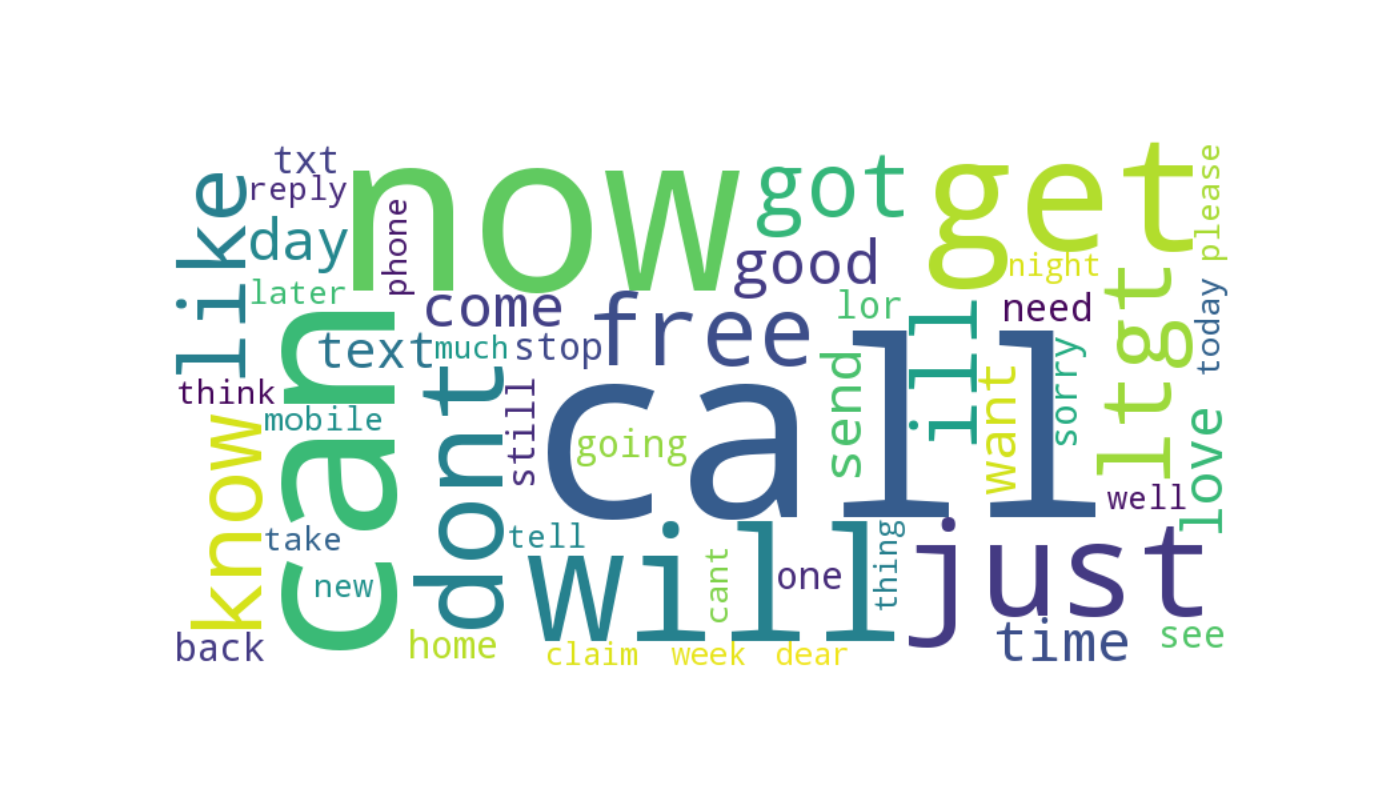
\includegraphics[width=\textwidth]{word_cloud.png}
    \caption[Figura simples]{Nuvem com as 50 palavras mais frequentes dentro de um universo de 
    palvras mais comuns de \texttt{SMS}.}
    \label{fig:wordcloud}
\end{figure}


 
\end{document}


